\documentclass[10pt,letterpaper,twocolumn]{article}

%2012-10-01 - Document préparé par David Lafrenière, pour le cours PHY3040.

%Pour langue et caractères spéciaux
\usepackage[french]{babel} 
\usepackage[T1]{fontenc}
\usepackage{lmodern}
\usepackage[utf8]{inputenc}

\usepackage[backend=biber, style=nature]{biblatex}
\addbibresource{reference.bib}

%Package for math expression
\usepackage{amsmath}
\usepackage{amsthm,amstext,amsfonts,bm,amssymb,amsthm}
\usepackage{mathtools}
\usepackage{bm}
\usepackage{gensymb}
\usepackage{mathrsfs}
\usepackage{physics}

%Package for drawings
\usepackage{tikz}
\usetikzlibrary{calc,patterns,angles,quotes}
\usepackage[compat=1.1.0]{tikz-feynman}
\usetikzlibrary{3d}
\usetikzlibrary{decorations.pathreplacing}
\usepackage{lineno}

%Package pour les symbole astronomiques
%\usepackage{wasysym}

\usepackage{hyperref}

%Pour ajuster les marges
\usepackage[top=2cm, bottom=2cm, left=2cm, right=2cm, columnsep=20pt]{geometry}

% Pour la commande onecolabstract (résumé 1 pleine largeur)
\usepackage{abstract}
	\renewcommand{\abstractnamefont}{\normalfont\bfseries}
	\renewcommand{\abstracttextfont}{\normalfont\itshape}

% Pour les titres de section/sous-section
\usepackage[compact]{titlesec}
\titleformat{\section}{\large\bfseries}{\thesection}{1em}{}
\titleformat{\subsection}{\normalsize\bfseries}{\thesubsection}{1em}{}
\titleformat{\subsubsection}{\normalsize}{\thesubsubsection}{1em}{}

%Package for graphic expression
\usepackage{graphicx}
\usepackage{wrapfig}
\usepackage{float}
\usepackage{caption}
\usepackage{subcaption}
\usepackage{enumitem}

\usepackage{booktabs,array}
\def\Midrule{\midrule[\heavyrulewidth]}
\newcount\rowc

\makeatletter
\def\ttabular{%
\hbox\bgroup
\let\\\cr
\def\rulea{\ifnum\rowc=\@ne \hrule height 1.3pt \fi}
\def\ruleb{
\ifnum\rowc=1\hrule height 1.3pt \else
\ifnum\rowc=6\hrule height \heavyrulewidth 
   \else \hrule height \lightrulewidth\fi\fi}
\valign\bgroup
\global\rowc\@ne
\rulea
\hbox to 10em{\strut \hfill##\hfill}%
\ruleb
&&%
\global\advance\rowc\@ne
\hbox to 10em{\strut\hfill##\hfill}%
\ruleb
\cr}
\def\endttabular{%
\crcr\egroup\egroup}

%Shorthand for space and some math expressions
\newcommand{\s}{\hspace{0.1cm}}
\renewcommand{\Im}{\operatorname{\mathbb{I}m}}
\renewcommand{\Re}{\operatorname{\mathbb{R}}}
%Shorthand for partial differential
\newcommand{\partialD}[2]{\frac{\partial #1}{\partial #2}}
%Shorthand for \left(\right)
\DeclarePairedDelimiter\autobracket{(}{)}
\newcommand{\br}[1]{\autobracket*{#1}}

\newcommand{\pyoutput}[2]{#2} % Simply output #2, use #1 as tag for python reader

%pour tableaux deluxetable
%\usepackage{deluxetable}

%Pour inclure des adresse web
\usepackage{url}

%Titre
\title{\vspace{-10mm}\Large
Fibres optiques%%%***éditer cette ligne***
\vspace{-4mm}}
\newcommand{\na}{\text{N.A.}}


%Auteur
\author{\large
Alexandre Adam
}
\date{\vspace{-8mm}}
\captionsetup{labelfont=bf, format=plain, font=footnotesize}
\begin{document}

\twocolumn[
\maketitle
\begin{onecolabstract} % 10 points
Six modes ont étés observés avec la fibre monomodes III (fibre A) en utilisant un laser GaN de longueur d'onde $\lambda = 405\s nm$. Quatre modes sont observés avec la fibre monomode II (fibre B), incluant le mode $LP_{02}$. Ces observations sont supplées par la mesure de l'ouverture numérique de la fibre A ($\na = 0.203 \pm 0.002$) et de la fibre B ($\na =  0.128 \pm  0.002$). Cette mesure est aussi performée pour une fibre multimode ($\na = 0.232 \pm 0.007$), pour laquelle on mesure l'atténuation à trois longueurs d'ondes différentes. On trouve que la fibre multimode ne peut pas être utilisée pour les communications longue distance. 
\vspace{4mm} %
\end{onecolabstract}
]

\section{Introduction}\label{intro} % 5 points
C'est en 1897 que Lord Rayleigh investigue pour la première fois la propagation d'ondes électromagnétiques dans un cylindre métallique vide, ainsi que ses différents modes de propagation. Sa découverte est oubliée pendant presque 40 ans, après quoi George C. Southworth et Wilmer L. Barrow redécouvre ce phénomène dans la même période de temps, entre 1931 et 1936\supercite{Packard1984}. \par
Les fibres optiques jouent aujourd'hui un rôle important dans la communication d'un signal sur de longues distances. Pour communiquer beaucoup d'information, une fibre doit transmettre des ondes dans le domaine du visible avec un faible coefficient d'atténuation. \par
Dans ce laboratoire, on s'intéresse à la propagation des ondes électromagnétiques dans des fibres à saut d'indice avec un c\oe{}ur fait de polymère. En particulier, on veut caractériser l'ouverture numérique et mesurer la forme du champ électrique transverse des différents modes de propagations. \par
On s'intéresse aussi au coefficient d'atténuation pour trois longueurs différentes dans le visible, de sortes qu'on puisse établir le type d'utilisation possible de la fibre optique de plastique.

\section{Théorie}\label{sec:theorie} % 10 points
\subsection{Propagation}\label{sec:thProp}
Selon le point de vue de l'optique géométrique, une fibre optique de section circulaire guide une onde électromagnétique dans son c\oe{}ur par réflexion totale interne. L'indice de réfraction du matériel diélectrique du c\oe{}ur $n_c$ doit être supérieur à l'indice de réfraction du revêtement $n_c > n$. Ainsi, il existe un angle critique $\phi_c$ déterminé par la loi de Snell-Descartes
\begin{equation}\label{eq:angleCritique}
	\phi_c = \sin^{-1}\br{\frac{n}{n_c}}
\end{equation}
tels que un rayon lumineux entrant dans le c\oe{}ur sera totalement réfléchit si son angle d'entrée par rapport à la normale de la section circulaire du fil est inférieur à un angle maximal $\theta_m$. On définit l'ouverture numérique\supercite{Pedrotti}
\begin{equation}\label{eq:nath}
	\na = n_{air} \sin \theta_m = n_c\cos \phi_c = \sqrt{n_c^2 - n^2}.
\end{equation}\par
La description des modes de propagations nécessite de résoudre les équations de Maxwell en utilisant l'approximation d'une fibre faiblement guidante\supercite{Snitzer1961,Gloge1971} ($\frac{n_c - n}{n} \ll 1$). Cette approximation permet de simplifier la description des modes permis dans la fibre par des modes linéairement polarisés $LP_{lm}$, qui sont une forme dégénérée des modes hybrides (\textit{c-à-d} des modes ayant une composante électrique et magnétique dans l'axe de la fibre).
Les champs électriques et magnétiques des modes $LP_{lm}$ peuvent s'exprimer en terme des fonctions de Bessel de première espèce à l'intérieur du c\oe{}ur $J(\frac{ur}{a})$  et en terme de des fonctions modifiées de Hankel dans le revêtement $K(\frac{wr}{a})$ où les paramètres $u$ et $w$ sont définis comme
\begin{align}
	u &= a\sqrt{(k^2n_c^2 - \beta^2)}, \\
	w &= a\sqrt{\beta^2 - k^2n^2}.
\end{align}
On a définit le paramètre $a$ comme le rayon du c\oe{}ur, $k = \frac{2\pi}{\lambda}$ et $\beta$ est la constante de propagation. Pour de petites valeurs de la fréquence normalisée\supercite{Gloge1971}
\begin{equation}\label{eq:V}
	v = ak\na,
\end{equation}
on obtient une approximation pour le paramètre $u(v)$ pour chaque mode ($v \ge u_c$)
\begin{equation}\label{eq:uplus}
	u(v) \simeq u_c \exp\left\{\frac{1}{s}\br{\arcsin{\br{\frac{s}{u_c}}} - \arcsin(\frac{s}{v})}     \right\},
\end{equation}
où 
\begin{equation}
	s = \sqrt{u_c^2 - l^2 - 1}
\end{equation}
et où $u_c$ est la m$^{\text{ième}}$ racine de $J_{l-1}(u)$. Cette approximation échoue pour le mode $LP_{01}$, pour lequel on utilise le résultat\supercite{Gloge1971}
\begin{equation}\label{eq:u0}
	u(v) = \frac{(1 + \sqrt{2})v}{1 + \sqrt[4]{4 + v^4}}.
\end{equation}
Notons de plus que $J_{-1}(u) = -J_1(u)$. On compte la racine $J_{1}(0) = 0$ ($m=1$) pour ce cas particulier. \par
Avec les solutions \eqref{eq:uplus} et \eqref{eq:u0}, on peut calculer la constante de propagation normalisée
\begin{equation}
	b(v) = 1 - \frac{u(v)^2}{v^2}
\end{equation}
qui décrit la propagation de chaque mode dans la fibre. En particulier, lorsque $b=0$ le mode est interdit.\par

Une solution graphique de la Figure \ref{fig:th1} nous permet alors de déterminer les modes permis pour un nombre $v$ particulier.
%(\textit{c.-à-d.} pour un faisceau monochromatique et une fibre de rayon \textit{a} particulière). 
\begin{figure}[H]
	\centering
	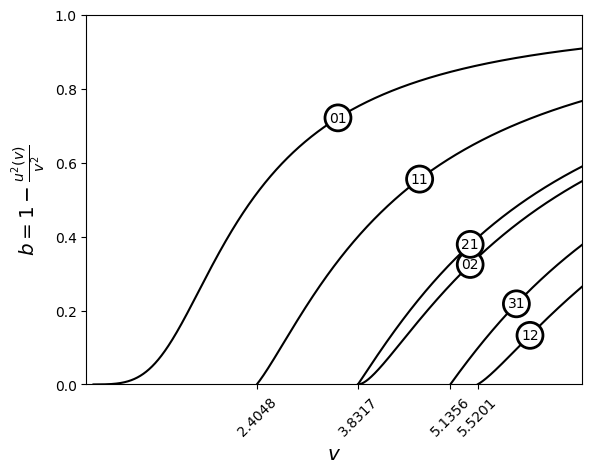
\includegraphics[width=\linewidth]{figures/theory.png}
	\caption{Constante de propagation normalisé $b(v)$ en fonction de la fréquence normalisée. Pour un nombre $v$ particulier, on peut déterminer le nombre de modes attendus en traçant une ligne verticale et en comptant les modes interceptés pour un $v$ donné. Les fréquences de coupures $v = u_c$ correspondent au zéros de la fonction de Bessel $J_{l-1}(u)$.}
	\label{fig:th1}
\end{figure}\par
L'intensité du champ électrique transverse à l'intérieur de la fibre sera mesurée par des détecteur CCD à la sortie de la fibre pour les fibres monomodes. Pour un mode $LP_{lm}$, le champ transverse prend la forme\supercite{Gloge1971}
\begin{equation}\label{eq:CTransverse}
	E_t(r, \phi) = \frac{J_l\br{\frac{ur}{a}}}{J_l(u)} \cos\br{l\phi},\hspace{0.3cm} \{r < a\}
\end{equation}
L'image d'un mode $l=0$ possède une symétrie azimutale avec des anneaux d'interférence destructive aux zéros de la fonction $J_1\br{\frac{ur}{a}}$. Le nombre d'anneau est égal à $m-1$. Les modes $l=1$ ont la caractéristique distinctive d'une ligne d'interférence destructive pour $\phi = \frac{\pi}{2}$ ou $\phi=0$ (le choix de la base $\cos\br{l\phi}$ ou $\sin\br{l\phi}$ est arbitraire). Ces modes possèdent des anneaux noirs aux zéros de la fonction $J_0$. Et ainsi de suite pour les modes $l=2,\s 3,\s\dots$
% exprimée en terme de la fréquence normalisé $V$
\subsection{Atténuation}

%Différents mécanismes d'atténuations ont pour rôle de diminuer l'intensité lumineuse. 
La loi empirique de Beer-Lambert permet de comprendre l'atténuation en terme d'un coefficient d'atténuation spécifique $\kappa_\lambda$, tels que\supercite{Pedrotti}
\begin{equation}\label{eq:BeerLambert}
	\kappa_\lambda = \frac{10}{L}\log_{10}\br{\frac{P_1}{P_2}},\s\s\s [dB\s km^{-1}]
\end{equation}
où $L$ est longueur parcourue par la lumière dans le milieu et $P_i$ est la puissance lumineuse mesurée aux deux extrémités de $L$. La description de $\kappa_\lambda$ est holistique, dans le sens où on ne distingue pas les mécanismes intrinsèques ou extrinsèques responsables de l'atténuation. 

\section{Méthodologie}\label{sec:metho} % 15 points


\subsection{Identification des fibres}\label{sec:IndentificationFibre}
On doit identifier trois fibres par les caractéristiques fournies par le manufacturier dans la Table \ref{tab:Manuf} 
\begin{table}[H]
	\centering
	\caption{Caractéristiques du manufacturier des fibres utilisées en laboratoire}
	\label{tab:Manuf}
	\begin{tabular}{|c|c|c|}
	\hline
		Fibre & $a$ ($\mu m$) & $\na$ \\\hline
		Multimode & 52.5 & 0.22 \\\hline
		Monomode I & 1.75 & 0.13 \\\hline
		Monomode II & 2.2 & 0.13 \\\hline
		Monomode III & 1.8 & 0.20\\\hline
	\end{tabular}
\end{table}
Pour distinguer les fibres monomodes, on utilise deux lasers: un laser He-Ne ($\lambda = 632.8\s nm$) de couleur rouge et un laser GaN de couleur mauve ($\lambda=405\s nm$). On peut alors distinguer les fibres qui ont la même $\na$ à partir de la Table \ref{tab:VNumber}.
\begin{table}[H]
	\centering
	\caption{Nombre $v$ calculé à partir de l'équation \eqref{eq:V} et de la Table \ref{tab:Manuf}}
	\label{tab:VNumber}
	\begin{tabular}{|c|c|c|}
	\hline
			Fibre & $v(\lambda = 632.8\s nm$) & $v(\lambda=405\s nm)$ \\\hline
			Monomode I & 2.259 & 3.529 \\\hline
			Monomode II & 2.840 & 4.437 \\\hline
			Monomode III &  3.574 &  5.585\\\hline
	\end{tabular}
\end{table}
 Ces nombres $v$ nous permettent de déterminer les modes présents par la solution graphique de la Figure \ref{fig:th1}. 
% On remarque qu'on peut identifier la monomode I si on n'observe que le mode $LP_{01}$ avec le laser rouge; on peut aussi identifier la fibre III si on observe les modes $LP_{31}$ et $LP_{12}$ avec le laser mauve. 


\subsection{Mesure de $\na$}\label{sec:mesureDeNa}
%Pour mesurer l'ouverture numérique d'une fibre multimode, on couple le laser He-Ne à la fibre. 
Comme la largeur du c\oe{}ur d'une fibre multimode est relativement large, l'intensité et la taille du faisceau émergent permettent de calculer l'ouverture numérique à partir de la mesure du diamètre $d$ du cercle projetté sur l'écran  par la fibre:
\begin{equation}\label{eq:na}
	\na = n_{air}\sin\br{\tan^{-1}\br{\frac{d}{2x}}} \underbrace{\simeq}_{\theta \ll 1} \frac{d}{2x},
\end{equation}
où $x$ est la distance entre la fibre et l'écran.\par
Dans le cas des fibres monomodes, on utilise un capteur CMOS Thorlabs pour mesurer la largueur du mode $LP_{01}$. En première approximation, ce mode est un pic gaussien. L'ajustement d'une courbe gaussienne sur le profil d'intensité nous permet de mesurer la largeur du pic. Le pic se termine là où l'intensité atteint 5\% de sa valeur maximale. \par 
%Comme on ne peut pas mesurer directement la distance de la fibre à la caméra, on utilise une vis micrométrique pour déplacer le détecteur. Ces trois mesures nous permettent d'inférer la distance $x$.
\subsection{Montage}
Les éléments principaux du montage sont dépictés dans la Figure \ref{fig:montage}.
\begin{figure}[H]
	\centering
	\begin{tikzpicture}
		\draw (-0.5, 0.5) rectangle (1, -0.5) node[pos=.5] {Laser};
		\draw[color=red] (1, 0.1) -- (2, 0.1);
		\draw[color=red]  (1, -0.1) -- (2, -0.1);
		
		\draw[<->] (2, -0.5) -- (2, 0.5);
		\draw[<->] (2.5, -0.5) -- (2.5, 0.5);
		
		\draw[color=red]  (2, 0.1) -- (2.5, -0.2);
		\draw[color=red]  (2, -0.1) -- (2.5, 0.2);
		\draw[color=red]  (2.5, -0.2) -- (2.7, 0.1);
		\draw[color=red]  (2.5, 0.2) -- (2.7, -0.1);
		
		\node at (2, -1) {Oculaire};
		\node at (2.5, 1) {Objectif};
		
		\draw[line width=0.25mm, color=red] (2.7, 0) ellipse (0.06 and 0.1);
		\draw[line width=0.25mm, color=red] (2.7, 0.1)[rounded corners] -- (3.2, 0.1) [rounded corners] -- (4, -0.9)[rounded corners] -- (5, 0.1)
																								[rounded corners] -- (5.5, 0.1);
		\draw[line width=0.25mm, color=red] (2.7, -0.1)[rounded corners] -- (3.2, -0.1) [rounded corners] -- (4, -1.1)[rounded corners] --  (5, -0.1)
																								[rounded corners] -- (5.5, -0.1);
		\draw (2.7, 0) ellipse (0.1 and 0.2);
		\draw (2.7, 0.2) -- (3.2, 0.2);
		\draw (2.7, -0.2) -- (3.2, -0.2);
		\draw (3.2, 0) ellipse (0.1 and 0.2);
		\node at (3, -0.5) {P};
		\draw[line width=0.25mm, color=red] (5.5, 0) ellipse (0.06 and 0.1);
		\draw (5.5, 0) ellipse (0.1 and 0.2);
		\draw (5, 0) ellipse (0.1 and 0.2);
		\draw (5, 0.2) -- (5.5, 0.2);
		\draw (5, -0.2) -- (5.5, -0.2);
		\begin{scope}[canvas is yz plane at x=6]
		   \draw[red, fill=red] (0,0) circle (0.3);
		   \draw (-0.75,0.75) rectangle (0.75,-0.75);
		\end{scope}
		\node at (6, -1.2) {Écran;};
		\node at (6, -1.55) {Détecteur CCD;};
		\node at (6, -1.9	) {Photodiode};
	\end{tikzpicture}
	\caption{Montage de l'expérience. Un laser de longueur d'onde $\lambda$ est couplé à la fibre (cylindre rouge gras) supporté par une plateforme mobile P. Cette plateforme possède deux degrés de libertés en \textit{x} et \textit{y} pour maximiser le couplage et isoler les modes $LP_{lm}$. Le faisceau est guidé par la fibre jusqu'au détecteur. Le détecteur CCD est monté sur une plateforme mobile avec une vis micrométrique}
	\label{fig:montage}
\end{figure}
L'écran de la Figure \ref{fig:montage} est remplacé par un détecteur CCD pour les mesures faites sur les fibres monomodes. Comme la taille du faisceau à la sortie de ces fibres est seulement de quelques millimètres, on utilise un détecteur CCD qui nous permet de caractériser la géométrie du faisceau à la sortie avec une précision de $5.75\s \mu m$, soit la taille d'un pixel du capteur CMOS Thorlabs.\par
Pour s'assurer que le couplage laser/fibre est maximal (alignement du montage), on utilise une photodiode connecté à un picoampèremètre Keithley 6485 pour mesurer la puissance de sortie. 
\subsection{Observations des modes $LP_{lm}$}
Les fibres monomodes ont une quantité suffisamment faible de modes permis, de sortes qu'on peut les distinguer à l'aide d'un capteur CCD à la sortie de la fibre. Pour isoler un mode, on doit ajuster la position de l'entrée de la fibre à l'aide de la plateforme mobile de la Figure \ref{fig:montage} pour changer l'angle d'entré des rayons principaux. Ceci a pour effet de changer l'intensité de certains modes.
\subsection{Mesure du coefficient d'atténuation}\label{sec:attenuation}
La mesure de la puissance à l'extrémité de deux fibres de différentes longueurs permet de mesurer le coefficient $\kappa_\lambda$ de l'équation \ref{eq:BeerLambert}. On utilise les laser rouge et mauve mentionnés dans la section \ref{sec:IndentificationFibre}, en plus d'un laser He-Ne vert, $\lambda = 543.5\s nm$. \par
La puissance est lue sur le picoampèremètre connecté à la photodiode, sous la forme d'un courant photoélectrique. 

\section{Résultats et discussion}\label{sec:resultats} % 25 points
\subsection{Ouverture numérique}
L'écran est placé à $14.4 \pm 0.2 \s cm$ de la seconde extrémité de la fibre multimode couplée au laser. On observe un cercle de diamètre $6.7 \pm 0.1\s cm$ sur l'écran, ce qui permet de calculer l'ouverture numérique avec l'équation \eqref{eq:na}. En utilisant $n_{air} \simeq 1$ et l'approximation des petits angles, $\na = 0.232 \pm 0.007$. \par
La valeur du manufacturier (Table \ref{tab:Manuf}) est à l'intérieur de deux déviations standards de la valeur expérimentale. \par
Pour les fibres monomodes, on analyse le profil du mode $LP_{01}$ avec le laser rouge par l'ajustement d'une courbe gaussienne. Avec la définition de la largeur du pic à la section \ref{sec:mesureDeNa}, on peut déterminer le rayon de l'image en fonction du paramètre $\sigma$ de la gaussienne (déviation standard), sachant que la taille d'un pixel de la caméra est $5.75\s \mu m$:
\begin{equation}
	r = \sigma \sqrt{\ln(20)}\s\s\s [\mu m]
\end{equation}\par
Comme on ne peut mesurer directement la distance entre la fibre et le détecteur $x$, on utilise la vis micrométrique (voir la description du montage de la Figure \ref{fig:montage}) pour déplacer le détecteur sur la plateforme mobile d'une distance $\delta$ et on prend plusieurs images pour mesurer $r(\delta)$. Dans ce cas, on peut estimer l'ouverture numérique en ajustant une droite sur la fonction $r(\delta)$ dérivée de l'équation \eqref{eq:na}: $r(\delta) = \delta\na + b$ . Les résultats sont compilés dans la Table \ref{tab:NAMono}  

\begin{table}[H]
	\centering
	\caption{Ouverture numérique des fibres monomodes}
	\label{tab:NAMono}
	\begin{tabular}{|c|c|c|}
	\hline
			& Monomode A & Monomode B \\\hline
	$\na$ 	& $ 0.203 \pm 0.002$ & $ 0.128 \pm  0.002$ \\\hline
	\end{tabular}
\end{table}
On peut déjà identifier la monomode A comme étant la monomode III (Table \ref{tab:Manuf}). On doit analyser les modes permis de la monomode B pour correctement l'identifier.

\subsection{Modes}
%La fibre multimode possède\supercite{Pedrotti} ${m_{tot} \simeq \frac{2a}{\lambda}\na + 1}$ modes, soit ${\ge37}$ pour cette fibre (considérant les longueurs d'ondes laser utilisées).\par 
Pour la fibre monomode A, on observe les modes présentés à la Figure \ref{fig:MONOA}. La présence des modes $LP_{31}$ et $LP_{12}$ avec le laser mauve révèle que cette fibre est la monomode III, qui est la seule fibre avec une fréquence normalisée pour laquelle ces modes sont permis (Table \ref{tab:VNumber}) à $\lambda = 405\s nm$. Cette observation concorde avec la mesure de l'ouverture numérique (Table \ref{tab:NAMono}).
\begin{figure}[H]
	\centering
	\begin{subfigure}[t]{0.3\linewidth}
		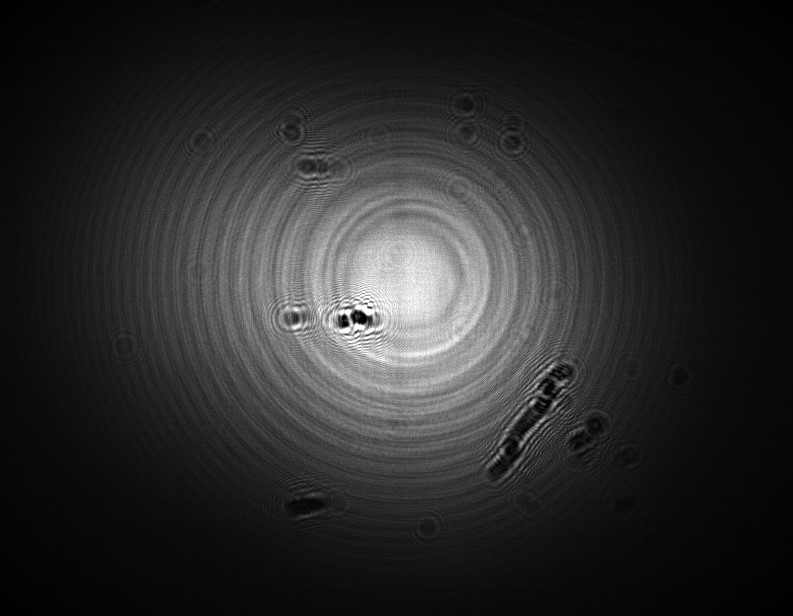
\includegraphics[height=1.7cm, width=\linewidth]{figures/mono-LP01-rouge.jpg}
		\caption{Mode $LP_{01}$, ${\lambda=632.8\s nm}$. }
		\label{fig:monoALP01}
	\end{subfigure}
	\begin{subfigure}[t]{0.3\linewidth}
		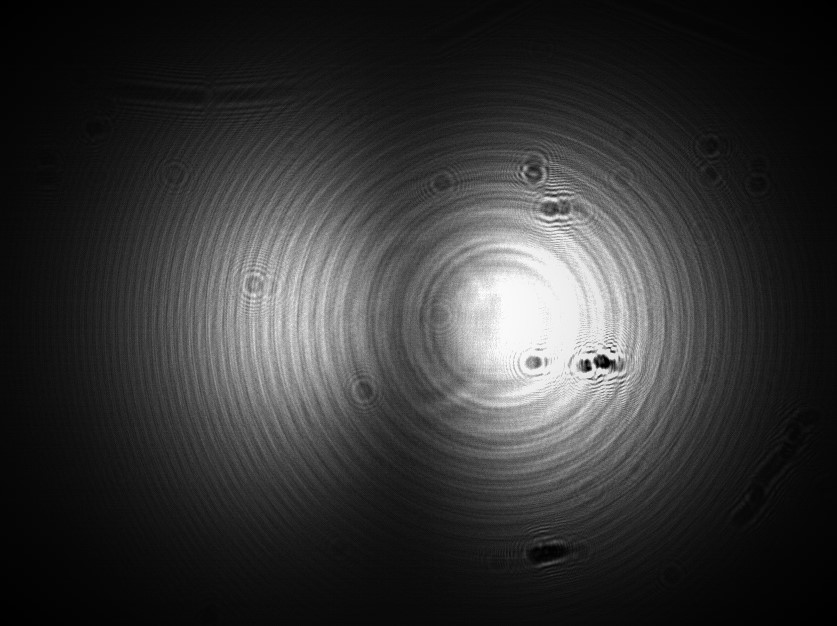
\includegraphics[height=1.7cm, width=\linewidth]{figures/monoA-LP11-rouge.jpg}
		\caption{Mode $LP_{11}$, ${\lambda=632.8\s nm}$.}
		\label{fig:monoALP11}
	\end{subfigure}
	\newline
	\begin{subfigure}[t]{0.3\linewidth}
		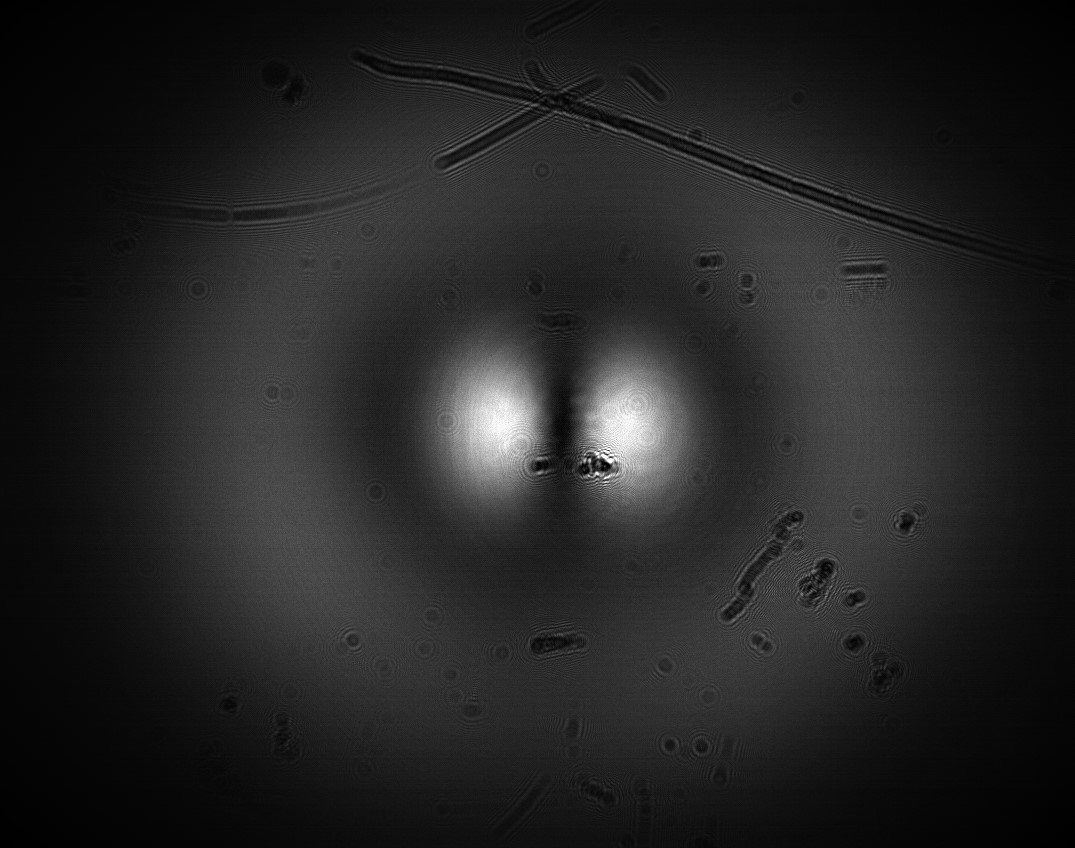
\includegraphics[height=1.7cm, width=\linewidth]{figures/A-LP12-mauv405.jpg}
		\caption{Mode $LP_{12}$, ${\lambda=405\s nm}$. }
		\label{fig:monoALP12}
	\end{subfigure}
	\begin{subfigure}[t]{0.3\linewidth}
		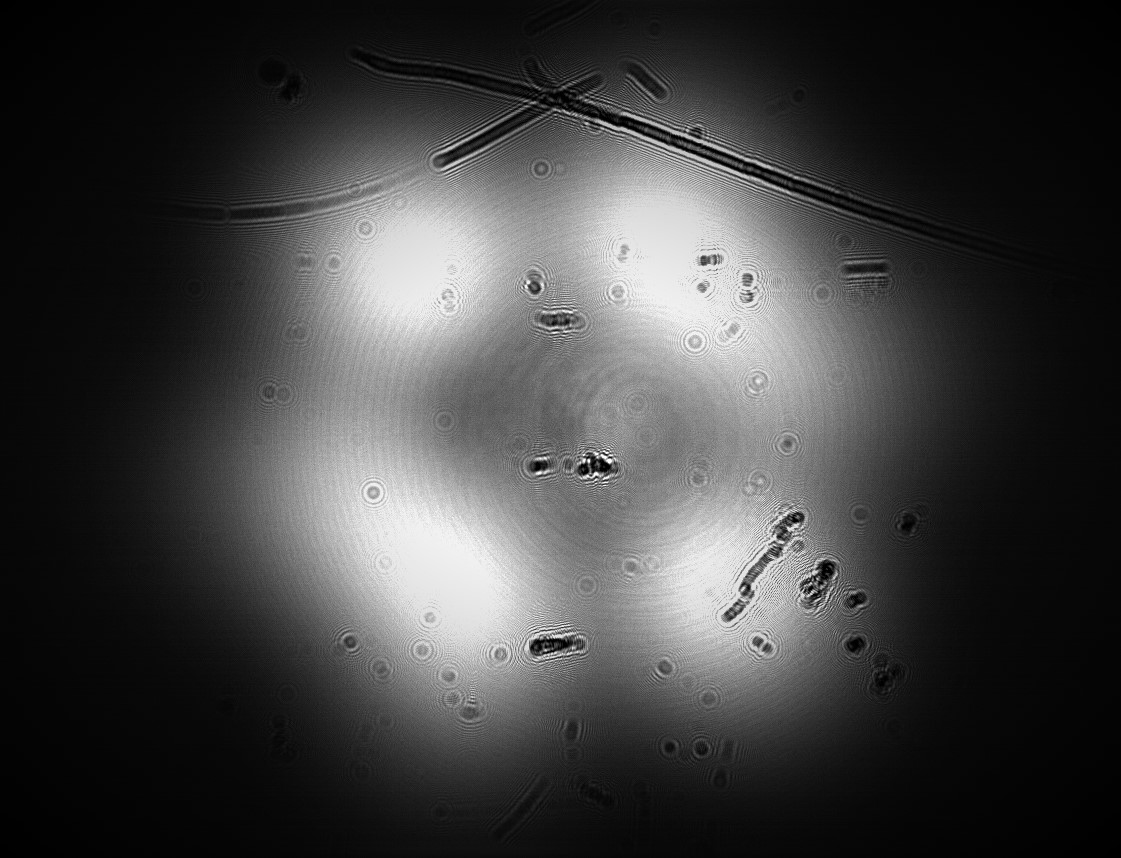
\includegraphics[height=1.7cm, width=\linewidth]{figures/A-LP21-mauve405(3).jpg}
		\caption{Mode $LP_{21}$, ${\lambda=405\s nm}$.}
		\label{fig:monoALP21}
	\end{subfigure}
	\begin{subfigure}[t]{0.3\linewidth}
		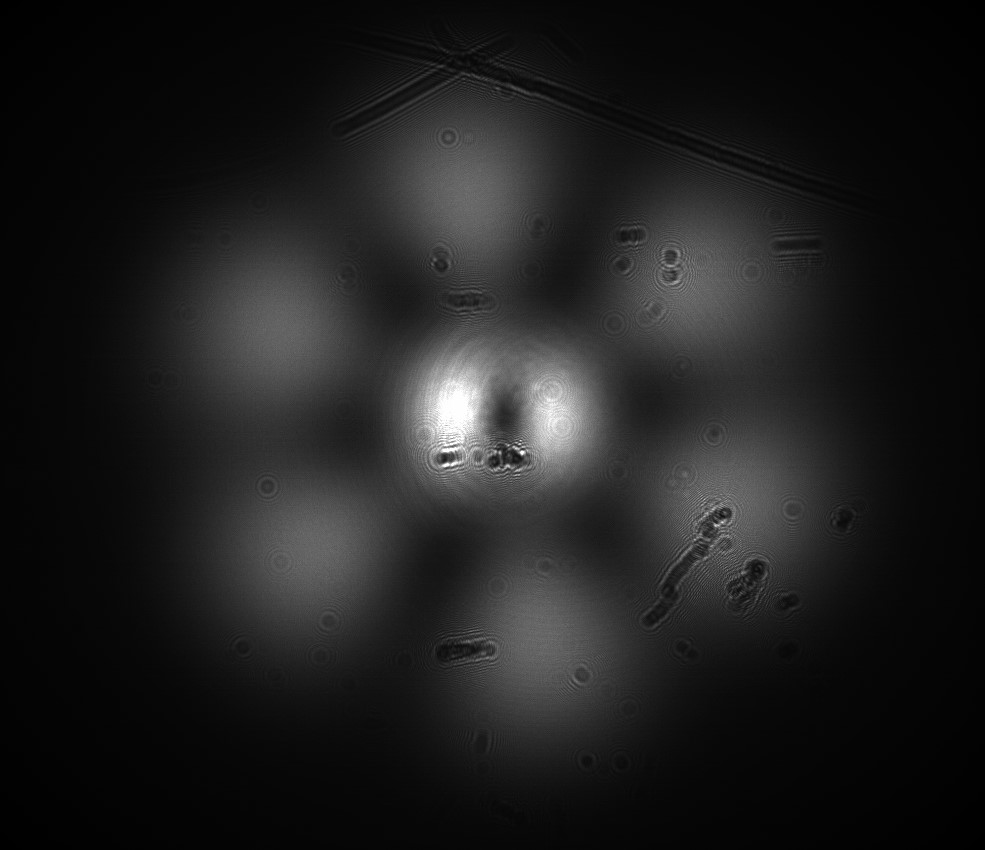
\includegraphics[height=1.7cm, width=\linewidth]{figures/A-LP31et12-mauve405.jpg}
		\caption{Superposition de $LP_{31}$ et $LP_{12}$, ${\lambda=405\s nm}$.}
		\label{fig:monoALP31et12}
	\end{subfigure}
	\caption{Modes de la fibre monomode A.}
	\label{fig:MONOA}
\end{figure}
Les deux premiers modes $LP_{01}$ et $LP_{11}$ sont obtenus avec $\lambda=632.8\s nm$, où les modes plus élevés sont interdits. Ceci permet de les isoler plus facilement avec le montage. Comme attendu, $LP_{01}$ (Figure \ref{fig:monoALP01}) prend la forme d'une tache circulaire, alors que $LP_{11}$ (Figure \ref{fig:monoALP11}) possède une ligne d'interférence destructrice verticale ($\phi=\frac{\pi}{2}$) distinctif du $\cos\phi$ dans l'équation \eqref{eq:CTransverse}. \par
Avec $\lambda=405\s nm$, le nombre $v=5.585$ (Table \ref{tab:VNumber}); 3 modes supplémentaires sont visibles. Le mode $LP_{12}$ (Figure \ref{fig:monoALP12}) possède la même ligne d'interférence visible dans la Figure \ref{fig:monoALP11}, avec l'addition d'un zéro de la fonction de Bessel sous la forme d'un anneau. Le mode $LP_{21}$ (Figure \ref{fig:monoALP21}) possède deux lignes d'interférences où $\cos(2\phi) = 0$, soit à $\phi=\frac{\pi}{4}$ et $\phi=\frac{3\pi}{4}$. \par
Finalement, le mode $LP_{31}$ (Figure \ref{fig:monoALP31et12}) est observé en superposition avec $LP_{12}$. Il nous était impossible d'isoler $LP_{31}$ puisque le croisement des trois lignes d'interférences ($\cos(3\phi)=0 \implies \phi \in \{\frac{\pi}{6},\s \frac{\pi}{2},\s \frac{5\pi}{6} \}$) crée une zone noire dans le centre de ce mode, où la lumière du mode fondamental et du mode $LP_{12}$ est le plus intense. \par

On observe les modes $LP_{21}$ et $LP_{02}$ pour la fibre B, ce qui révèle que c'est la monomode II. Selon la Table \ref{tab:VNumber} à $405\s nm$, elle se distingue de la monomode I pour laquelle $v< 3.8317$, le deuxième zéro de $J_1(u)$. La Figure \ref{fig:MONOB} montre trois modes observés avec le laser mauve. 
\begin{figure}[H]
	\centering
	\begin{subfigure}{0.3\linewidth}
		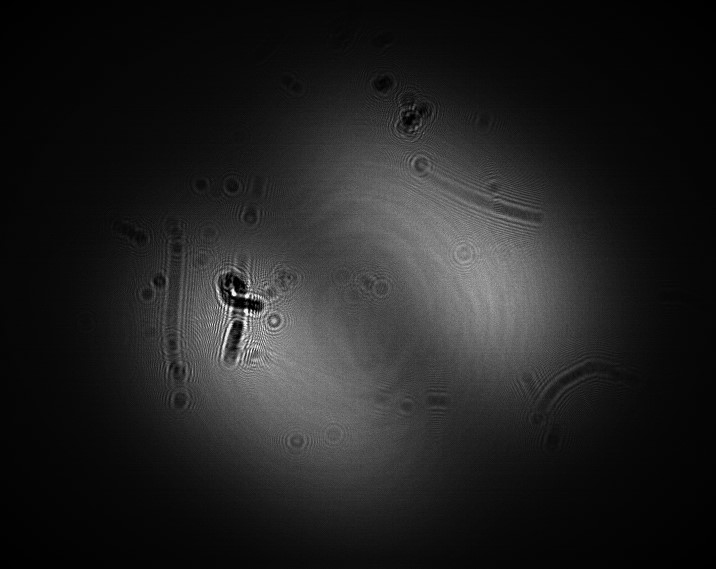
\includegraphics[height=2cm, width=\linewidth]{figures/monoB-BLUE-LP11(VRAI).jpg}
		\caption{Mode $LP_{11}$, ${\lambda=405\s nm}$.}
		\label{fig:monaBLP11}
	\end{subfigure}
	\begin{subfigure}{0.3\linewidth}
		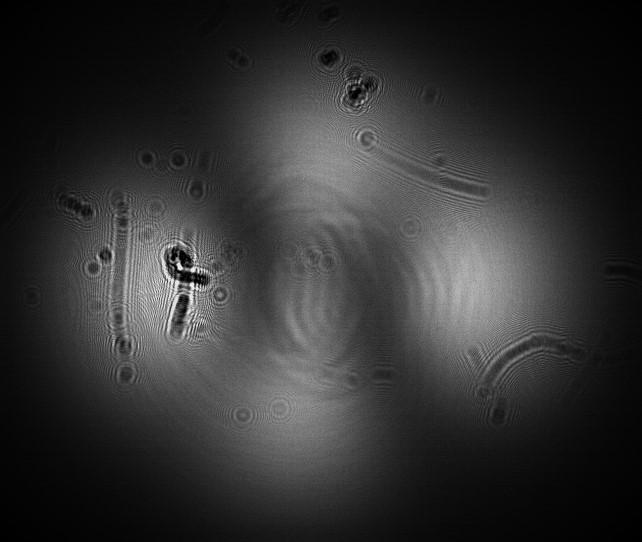
\includegraphics[height=2cm, width=\linewidth]{figures/monoB-BLUE-LP21.jpg}
		\caption{Mode $LP_{21}$, ${\lambda=405\s nm}$.}
		\label{fig:monaBLP21}
	\end{subfigure}
	\begin{subfigure}{0.3\linewidth}
		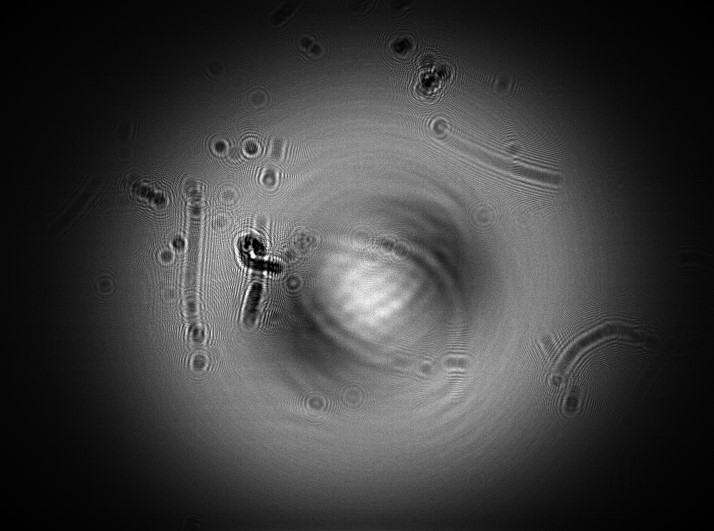
\includegraphics[height=2cm, width=\linewidth]{figures/monoB-BLUE-LP02.jpg}
		\caption{Mode $LP_{02}$, ${\lambda=405\s nm}$.}
		\label{fig:monaBLP02}
	\end{subfigure}
	\caption{Modes de la fibre monomode B.}
	\label{fig:MONOB}
\end{figure}
On observe encore les modes $LP_{11}$ et $LP_{21}$ (Figure  \ref{fig:monaBLP11} et \ref{fig:monaBLP21}), presque identiques aux Figures \ref{fig:monoALP11} et \ref{fig:monoALP21}. Le mode $LP_{02}$ était très difficile à détecter avec la fibre A. En effet, sa tache central était constamment brisée par la superposition avec le mode $LP_{12}$. Avec cette fibre, le mode $LP_{12}$ est interdit puisque $v<5.5201$ (voir Table \ref{tab:VNumber}), donc il est plus facile de l'isoler dans ce contexte. On remarque la présence d'un anneau, distinctif d'un mode $m=2$, et aucune ligne d'interférence (${l=0\implies \cos(l\phi) = 1}$).\par
Les observations faites sur les différents mode sont cohérentes avec la théorie décrite à la section \ref{sec:thProp}. 
\subsection{Coefficient d'atténuation}
Pour réaliser l'expérience décrite sommairement à la section \ref{sec:attenuation}, on a utilisé une fibre multimode de longueur $L_1 = 68.6 \pm 0.2\s cm$ et une deuxième avec $L_2 = 192.5\pm0.4\s cm$. \par
La mesure du courant photoélectrique à la sortie de la fibre est déterminé par la qualité du couplage laser/fibre. Dans chacun des cas, on cherche à maximiser la puissance fournie pour obtenir une mesure, mais cette méthode introduit une erreur aléatoire. On répète donc chacune des mesures (incluant le couplage) deux fois et on prend la moyenne comme résultat.\par
\begin{table}[H]
	\centering
	\caption{$\kappa_\lambda$ mesuré pour la fibre multimode.}
	\label{tab:kappa}
	\resizebox{\linewidth}{!}{
	\begin{tabular}{|c|c|c|c|}
	\hline
	$\lambda\s [nm]$ &  $405$ & $543.5$ & $632.8$ \\\hline
	$\kappa_\lambda \s [dB\s km^{-1}]$ & $46 \pm 0.5 \times 10^2$ & $6 \pm 2 \times 10^3$ & $39 \pm 4 \times 10^2$\\\hline
	\end{tabular}
	}
\end{table}
Les résultats de la Table \ref{tab:kappa} indique que le plastique qui compose les fibres optiques n'est pas très transparent pour les longueurs d'ondes considérées. L'erreur sur ces mesures est importante en raison de la méthode utilisée pour coupler le laser à la fibre. Notons aussi que la fibre était courbée dans le montage. Ceci induit des pertes supplémentaires telles qu'on ne peut établir de conclusion sur l'atténuation intrinsèque de la fibre. 

\section{Conclusion}\label{sec:conclusion} % 10 points
Nous avons identifier la fibre A comme étant la monomode III. Son ouverture numérique $\na = 0.203 \pm 0.002$ est en accord avec la valeur du manufacturier (Table \ref{tab:Manuf}) et les modes observés sont tels que prédis par la théorie des guide d'ondes faiblement guidant. La fibre B possède une ouverture numérique $\na = 0.128 \pm  0.002$. Les modes $LP_{02}$ et $LP_{21}$ indiquent alors que c'est la fibre monomode II via la fréquence normalisé (Table \ref{tab:VNumber}).\par
L'ouverture de la fibre multimode est mesuré: ${\na =  0.232 \pm 0.007}$, ainsi que l'atténuation à trois longueurs d'ondes différentes. Les valeurs de la Table \ref{tab:kappa} montrent que les pertes se situent entre $50\%$ et $60\%$ chaque mètre, rendant inutilisable cette fibre pour les communications longues distances. \par
Pour mieux caractériser l'atténuation de la fibre, il serait pertinent de comparer les nos résultats avec les prédictions théoriques de la théorie potentiel de Morse\supercite{Ishigure1995} et estimer l'apport extrinsèque des courbure dans la fibre à l'atténuation.
%Pour mieux caractériser l'atténuation, il serait intéressant de tester différentes courbure de fibre à chaque longueurs d'onde. 


\printbibliography

\end{document}
